\documentclass[aspectratio=169,10pt]{beamer}
\usepackage[T1]{fontenc}
\usepackage[utf8]{inputenc}
\usepackage{helvet,booktabs,tikz,amsmath,array}
\renewcommand{\familydefault}{\sfdefault}
\usetikzlibrary{arrows.meta,positioning}
\usetheme{Madrid}
\definecolor{ink}{HTML}{142C43}
\definecolor{accent}{HTML}{007F86}
\definecolor{soft}{HTML}{EDF5F5}
\setbeamercolor{structure}{fg=accent}
\setbeamercolor{frametitle}{bg=ink,fg=white}
\setbeamercolor{title}{bg=ink,fg=white}
\setbeamercolor{block title}{bg=accent!15,fg=ink}
\setbeamercolor{block body}{bg=soft,fg=ink}
\setbeamertemplate{navigation symbols}{}
\setbeamertemplate{footline}{\hspace{5mm}\scriptsize Photonic NPU\quad|\quad Development proposal\quad|\quad October 2026\hfill\insertframenumber\hspace{5mm}\vspace{3mm}}
\setlength{\tabcolsep}{5pt}
\newcolumntype{L}[1]{>{\raggedright\arraybackslash}p{#1}}
\pdfstringdefDisableCommands{\def\translate#1{#1}}
\newcommand{\stage}[1]{\par\vspace{2mm}{\footnotesize\color{accent}#1\par}}
\newcommand{\source}[2]{\vfill{\tiny Source: \href{#1}{#2}\par}}
% Generated by preseed_budget.py; amounts in USD.
\newcommand{\FundingAsk}{\$750k}
\newcommand{\CoreBudget}{\$650k}
\newcommand{\ReserveBudget}{\$100k}

\title{A Modular Photonic NPU}
\subtitle{Programmable optical computation with electronic control}
\author{Pavel Chekmaryov}
\institute{\href{mailto:p@occurai.com}{p@occurai.com}}
\date{October 2026}

\begin{document}

\begin{frame}
\titlepage
\centering
{\large A soliton microcomb supplies parallel channels.\\
A programmable optical core performs the computation.\par}
\vspace{4mm}
\textbf{\FundingAsk{} pre-seed}\quad|\quad15-month feasibility program
\end{frame}

\begin{frame}{First Workload: Repeated Inference}
\begin{block}{The use case we will test}
Repeated matrix--vector projections in a small inference model: one input vector at a time, with weights reused across a continuous stream.
\end{block}
\begin{itemize}
\item Prospective users: teams building real-time sensing and control hardware.
\item They need useful prediction accuracy within a defined response-time and power budget.
\item The opportunity depends on the complete system: loading inputs, computing, reading outputs, and applying the next operation.
\end{itemize}
\begin{exampleblock}{First commercial question}
Which recurring layer is important enough for a hardware team to evaluate a dedicated processor?
\end{exampleblock}
\stage{Initial application hypothesis. The task and buyer requirements will be selected during the first phase.}
\end{frame}

\begin{frame}{The Product: A Photonic Compute Core}
\centering
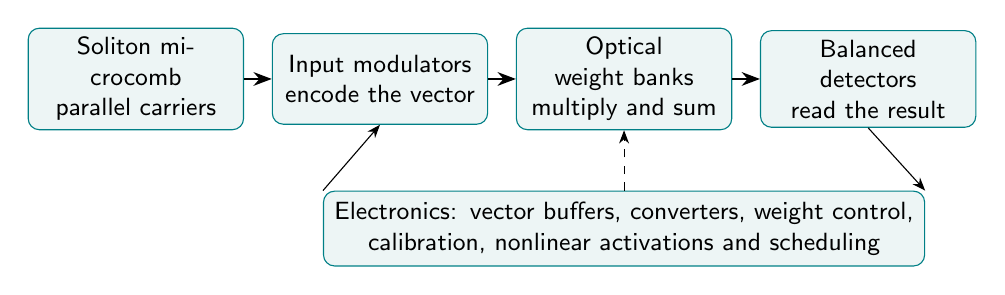
\begin{tikzpicture}[box/.style={draw=accent,rounded corners,fill=soft,align=center,text width=2.5cm,minimum height=1.15cm,font=\small},>=Stealth]
\node[box] (comb) at (0,0) {Soliton microcomb\\parallel carriers};
\node[box] (input) at (3.1,0) {Input modulators\\encode the vector};
\node[box] (weights) at (6.2,0) {Optical weight banks\\multiply and sum};
\node[box] (output) at (9.3,0) {Balanced detectors\\read the result};
\node[box,text width=7.4cm,minimum height=.95cm] (control) at (6.2,-1.9) {Electronics: vector buffers, converters, weight control,\\calibration, nonlinear activations and scheduling};
\draw[->,thick] (comb)--(input);
\draw[->,thick] (input)--(weights);
\draw[->,thick] (weights)--(output);
\draw[->] (control.north west)--(input.south);
\draw[->,dashed] (control.north)--(weights.south);
\draw[->] (output.south)--(control.north east);
\end{tikzpicture}
\par\vspace{3mm}
{\large Optical arithmetic: \(y=Wx\)\par}
\vspace{2mm}
The first chip we will fabricate is the compute core. Gen 1 uses an existing or shared microcomb source and external test electronics.
\stage{Proposed architecture. A later chiplet or SoC can integrate more of the system.}
\end{frame}

\begin{frame}{Useful Precision in One Pass}
\begin{block}{What we aim to improve}
Meet a chosen inference-accuracy requirement without repeating and averaging the same optical calculation.
\end{block}
\begin{columns}[T]
\begin{column}{.48\textwidth}
\textbf{Engineering work}
\begin{itemize}
\item Model source power, coupling loss and receiver noise together.
\item Set receiver gain and bandwidth for the actual vector rate.
\item Calibrate optical weights, signed readout and channel crosstalk.
\end{itemize}
\end{column}
\begin{column}{.48\textwidth}
\textbf{Why this could matter}
\begin{itemize}
\item Fewer repeated measurements could reduce latency and energy per useful result.
\item Reusing loaded weights could reduce repeated programming and data movement.
\item The gain must survive converter and control overhead.
\end{itemize}
\end{column}
\end{columns}
\stage{A testable design hypothesis. The noise model and bench measurements must establish the improvement.}
\end{frame}

\begin{frame}{First Hardware: An 8\(\times\)8 Test Tile}
\begin{columns}[T]
\begin{column}{.46\textwidth}
\begin{block}{Compute chip}
\begin{itemize}
\item Eight optical input channels and eight logical outputs.
\item Programmable weights; balanced readout for signed weights.
\item Monitor taps and calibration structures.
\item Repeated tiles with short receiver connections.
\end{itemize}
\end{block}
\end{column}
\begin{column}{.50\textwidth}
\small
\begin{tabular}{L{.29\textwidth}L{.58\textwidth}}
\toprule
\textbf{Part} & \textbf{Implementation}\\
\midrule
Source & Existing SiN soliton source; external pump\\[2mm]
Compute & Silicon-on-insulator modulators and weight banks\\[2mm]
Readout & Foundry-supported Ge/SiGe photodetectors\\[2mm]
Control & CMOS electronics; FPGA and SRAM during prototyping\\
\bottomrule
\end{tabular}
\end{column}
\end{columns}
\vspace{3mm}
\textbf{Starting band:} around 1550 nm, subject to source and foundry compatibility. The base round funds one new compute-chip fabrication.
\stage{8\(\times\)8 is a working prototype scale. Final dimensions, spacing and device choices require a foundry PDK and design review.}
\end{frame}

\begin{frame}{What the Prototype Must Establish}
\small
\begin{tabular}{L{.23\textwidth}L{.64\textwidth}}
\toprule
\textbf{Test} & \textbf{Working acceptance target / measurement}\\
\midrule
Optical arithmetic & \(\leq5\%\) normalized MVM error on a locked test set, in a single pass.\\[2mm]
Inference quality & \(\leq1\) percentage-point accuracy loss versus the same digital model on the chosen task.\\[2mm]
Latency and energy & Measure digital input-buffer to output-buffer time and total module power, including source, converters and controls.\\[2mm]
Repeatability & Repeat calibration, startup and sustained operation under defined laboratory conditions.\\[2mm]
Electronic baseline & Compare the same task with an optimized CPU and an appropriate FPGA or electronic NPU; include a GPU where relevant.\\
\bottomrule
\end{tabular}
\par
\vspace{2mm}
The tile validates the physical model. A measured small-tile result and a conservative scaling model guide the next processor.
\stage{Targets are proposed, not achieved. Lock the test protocol after the initial noise model and quotes, before fabrication.}
\end{frame}

\begin{frame}{Existing Work and Where We Must Add Value}
\begin{tabular}{L{.21\textwidth}L{.40\textwidth}L{.27\textwidth}}
\toprule
\textbf{Reference} & \textbf{What is already established} & \textbf{Our implication}\\
\midrule
Feldmann et al., 2021 & Soliton-microcomb photonic multiply--accumulate hardware. & The basic architecture has precedent.\\[2mm]
Meyer et al., 2026 & A reprogrammable \(9\times3\) microcomb processor; Enlightra contributes to the research. & Precision, readout and complete-system cost are relevant benchmarks.\\[2mm]
Hua et al., 2025 & Larger photonic--electronic compute integration for low-latency workloads. & Packaging and electronic support are part of the processor.\\
\bottomrule
\end{tabular}
\begin{block}{Our contribution must be demonstrated}
A specific readout, calibration or integration improvement that meets the chosen task's accuracy and operating budget.
\end{block}
\stage{Electronic NPUs and FPGAs are alternatives. Soliton use alone is not differentiation.}
\source{https://www.nature.com/articles/s41467-026-71599-2}{Meyer et al. (2026); Feldmann et al. and Hua et al. linked in the evidence appendix}
\end{frame}

\begin{frame}{First Customers and Commercial Path}
\begin{block}{Initial customer hypothesis}
Hardware teams with a recurring dense inference layer and a demanding response-time or energy budget. First discussions should establish the task, interface, accuracy and purchasing decision.
\end{block}
\begin{enumerate}
\item \textbf{Specify:} agree a representative workload and electronic baseline with a potential evaluator.
\item \textbf{Demonstrate:} test a packaged compute tile and its software interface.
\item \textbf{Evaluate:} obtain outside measurements and a defined next integration decision.
\item \textbf{Productize:} supply compute modules; pursue chiplet or IP integration when justified by demand.
\end{enumerate}
\stage{No customer agreement is claimed. Prices, unit volumes and production margins will follow an actual module specification and evaluation route.}
\end{frame}

\begin{frame}{15-Month Feasibility Program}
\begin{tabular}{L{.14\textwidth}L{.74\textwidth}}
\toprule
\textbf{Window} & \textbf{Deliverable and decision}\\
\midrule
M0--3 & Secure technical lead and lab/source access; obtain quotes; select task, accuracy target and comparison boundary.\\[2mm]
M3--6 & Build loss/noise model and electronic baseline; review PDK design and packaging; commit to fabrication only within the funded scope.\\[2mm]
M6--10 & Fabrication and assembly; prepare source, receiver, converters and test software in parallel.\\[2mm]
M10--13 & Bring up optical arithmetic; calibrate weights and readout; measure precision and stability.\\[2mm]
M13--15 & Run the locked task and outside review; estimate scaling and module cost; choose the next design or revise the architecture.\\
\bottomrule
\end{tabular}
\stage{Timing depends on foundry turnaround and equipment access. Begin follow-on discussions around M8--10; financing is not assumed.}
\end{frame}

\begin{frame}{Team and Starting Point}
\begin{block}{Pavel Chekmaryov --- Founder}
Experience at Snowcap Compute; exploratory work on topological features for machine learning, nonlinear-optics simulations and photonic layouts.
\end{block}
\begin{exampleblock}{Seeking a technical co-founder or photonics engineer}
Hands-on experience in photonic compute, foundry design, packaging and optical testing. Specialist electronics and test support are also required.
\end{exampleblock}
\begin{itemize}
\item Existing repository work supports exploration and preparation.
\item This NPU's arithmetic, power and latency remain to be measured.
\item Technical staffing, laboratory access and fabrication support are early execution milestones.
\end{itemize}
\stage{Advisor names and affiliations will be added after their role and public attribution are confirmed.}
\end{frame}

\begin{frame}{From Compute Tile to SoC}
\begin{enumerate}
\item \textbf{Test chip:} a small programmable optical computation with a defined error budget.
\item \textbf{Compute module:} larger or repeated tiles, memory, converters, software and a useful workload.
\item \textbf{Chiplet:} integration with a host processor through an agreed interface and packaging process.
\item \textbf{SoC:} integrate more of the optical computation with electronic memory and control.
\end{enumerate}
\begin{block}{The end goal}
A functioning photonic processor. Each generation must justify its precision, data movement, integration cost and application.
\end{block}
\stage{This round establishes the first tile and its scaling evidence. Later generations require additional design work and funding.}
\end{frame}

\begin{frame}{Funding Ask: \FundingAsk{} Pre-Seed}
\begin{columns}[T]
\begin{column}{.53\textwidth}
\centering\footnotesize
% Generated by preseed_budget.py.
\begin{tabular}{lr}
\toprule
\textbf{15-month allocation} & \textbf{USD}\\
\midrule
People / specialist support & \$280k\\
Compute-chip fabrication & \$120k\\
Packaging / assembly & \$70k\\
Electronics / shared lab & \$100k\\
Microcomb / pump / optics access & \$50k\\
Operations / IP & \$30k\\
Contingency reserve & \$100k\\
\midrule
\textbf{Total} & \textbf{\$750k}\\
\bottomrule
\end{tabular}

\end{column}
\begin{column}{.43\textwidth}
\begin{block}{What this round buys}
A custom compute-chip prototype, a controlled test system, precision and power measurements, one workload benchmark and outside technical review.
\end{block}
\textbf{\CoreBudget{} scheduled work}\\
\textbf{\ReserveBudget{} reserve}\\[3mm]
One new compute-chip run; an existing or shared soliton source; shared lab equipment; lean staffing.
\end{column}
\end{columns}
\vspace{3mm}
\textbf{Next financing milestone:} a measured tile, a credible scaled design and a defined customer evaluation.
\stage{Planning allocation in USD. Supplier quotes are required; the reserve does not guarantee a full respin.}
\end{frame}

\appendix

\begin{frame}{Appendix: Precision and Accuracy}
\begin{block}{Normalized matrix--vector error}
For a locked set of input vectors and reference results:
\[
\epsilon_{\rm MVM}
=\frac{\sum_i\lVert \hat y_i-Wx_i\rVert_2}
{\sum_i\lVert Wx_i\rVert_2}.
\]
\end{block}
\begin{itemize}
\item Record input distribution, weight range, signed encoding and calibration method.
\item Keep weight-programming levels, output numerical error and inference accuracy separate.
\item Report near-zero-output absolute errors and variation across channels.
\item If averaging is used, count all repeated measurements in latency and energy.
\end{itemize}
\stage{The working 5\% MVM and 1 percentage-point task targets are independent checks; neither implies a particular effective bit precision.}
\end{frame}

\begin{frame}{Appendix: Complete-System Measurement}
\begin{itemize}
\item Digital vector buffer to digital result buffer, with converter and receiver costs included.
\item Measure total electrical draw; separate pump, tuning, conversion, readout and control contributions.
\item Report host transfer time separately, then include it in the application comparison.
\item State weight-update time, input/output rate, calibration duty and operating conditions.
\end{itemize}
\begin{block}{Arithmetic throughput is only one metric}
For an \(N\)-input, \(M\)-output tile at \(r\) vectors/s:\\
\(NM r\) MAC/s, or \(2NM r\) operations/s when one MAC counts as two operations.\\[2mm]
An \(8\times8\) tile at a hypothetical 1 Gvector/s gives 0.128 TOPS gross. This does not specify precision, total power or application speed.
\end{block}
\stage{Model larger arrays using measured loss, noise, tuning and electrical overhead; do not extrapolate from passive optical arithmetic alone.}
\end{frame}

\begin{frame}{Appendix: Process and Integration Choices}
\begin{itemize}
\item \textbf{Source:} prefer an accessible SiN soliton source with a measured spectrum and power budget.
\item \textbf{Compute:} a qualified SOI process with modulators, detectors, filters and test structures.
\item \textbf{Packaging:} source and compute dies can remain separate in Gen 1; coupling loss and thermal conditions enter the error budget.
\item \textbf{Weights:} tunable elements first. Nonvolatile phase-change weights are a later option if programming, precision and endurance justify them.
\item \textbf{Alternatives:} assess AlGaAs or other platforms when a validated process and team access offer an actual advantage.
\end{itemize}
\stage{The repository's generic-PDK ring and retina layouts are historical experiments. A foundry-ready compute layout has not been established.}
\source{https://www.imec-int.com/en/press/imec-and-ghent-university-present-fully-integrated-single-chip-microwave-photonics-system}{Example silicon-photonics platform; exact access and device suitability require foundry confirmation}
\end{frame}

\begin{frame}{Appendix: Fabrication-Cost Sensitivity}
\centering
\begin{tabular}{rrr}
\toprule
\textbf{Fabrication only} & \textbf{Total with reserve} & \textbf{Gap above \FundingAsk}\\
\midrule
\$100k & \$730k & \$0\\
\$120k base & \$750k & \$0\\
\$200k & \$830k & \$80k\\
\$300k & \$930k & \$180k\\
\bottomrule
\end{tabular}
\par\vspace{4mm}
\raggedright
Other scheduled work stays at \$530k; packaging is already a separate \$70k allowance within that amount. The protected reserve remains \ReserveBudget{}.
\begin{block}{Before committing to tapeout}
Confirm foundry, packaging, source and test-equipment scope. If quotations exceed the allocation, revise scope or raise additional capital.
\end{block}
\stage{Sensitivity assumptions, not quotations. A second custom chip, dedicated laboratory or full respin requires a separate budget.}
\end{frame}

\begin{frame}{Appendix: Longer-Term Research}
\begin{block}{Topological representations for learning}
The founder's earlier work motivates experiments with topological descriptors. Current protein experiments do not establish an exact photonic E$_2$ or homotopy-group engine.
\end{block}
\begin{itemize}
\item \textbf{Exact algebra:} identify a specific operation and show how a physical circuit performs it correctly.
\item \textbf{Hopfions:} investigate an encoding and useful operation only after defining input, manipulation and readout.
\item \textbf{Photonic retina:} a possible later application of the processor, with a separate sensing and preprocessing architecture.
\end{itemize}
\stage{These directions motivate later research. The first NPU experiment is judged by arithmetic, task performance and complete-system cost.}
\end{frame}

\begin{frame}{Appendix: Evidence and Inputs to Complete}
\small
\begin{itemize}
\item \href{https://www.nature.com/articles/s41586-020-03070-1}{Feldmann et al., Nature (2021): soliton-microcomb tensor core}.
\item \href{https://www.nature.com/articles/s41467-026-71599-2}{Meyer et al., Nature Communications (2026): reconfigurable tensor processor}.
\item \href{https://www.nature.com/articles/s41586-025-08786-6}{Hua et al., Nature (2025): photonic--electronic accelerator}.
\item \href{https://www.nature.com/articles/s41467-023-38473-x}{Zhou et al., Nature Communications (2023): programmable photonic weight memory}.
\end{itemize}
\begin{block}{Company-specific inputs}
Technical-lead commitment; task and evaluator; loss/noise model; foundry and packaging quotes; source and lab access; measured prototype results; and ownership of the implementation.
\end{block}
\stage{Publications establish prior art. Company performance, customer demand and future sales remain to be established.}
\end{frame}

\end{document}
